\documentclass{article}

\usepackage{tikz}
\usepackage[inner=0.5cm,outer=0.5cm]{geometry}

\begin{document}
\subsection*{12 faces, 2nd type, wild}
 \bigskip

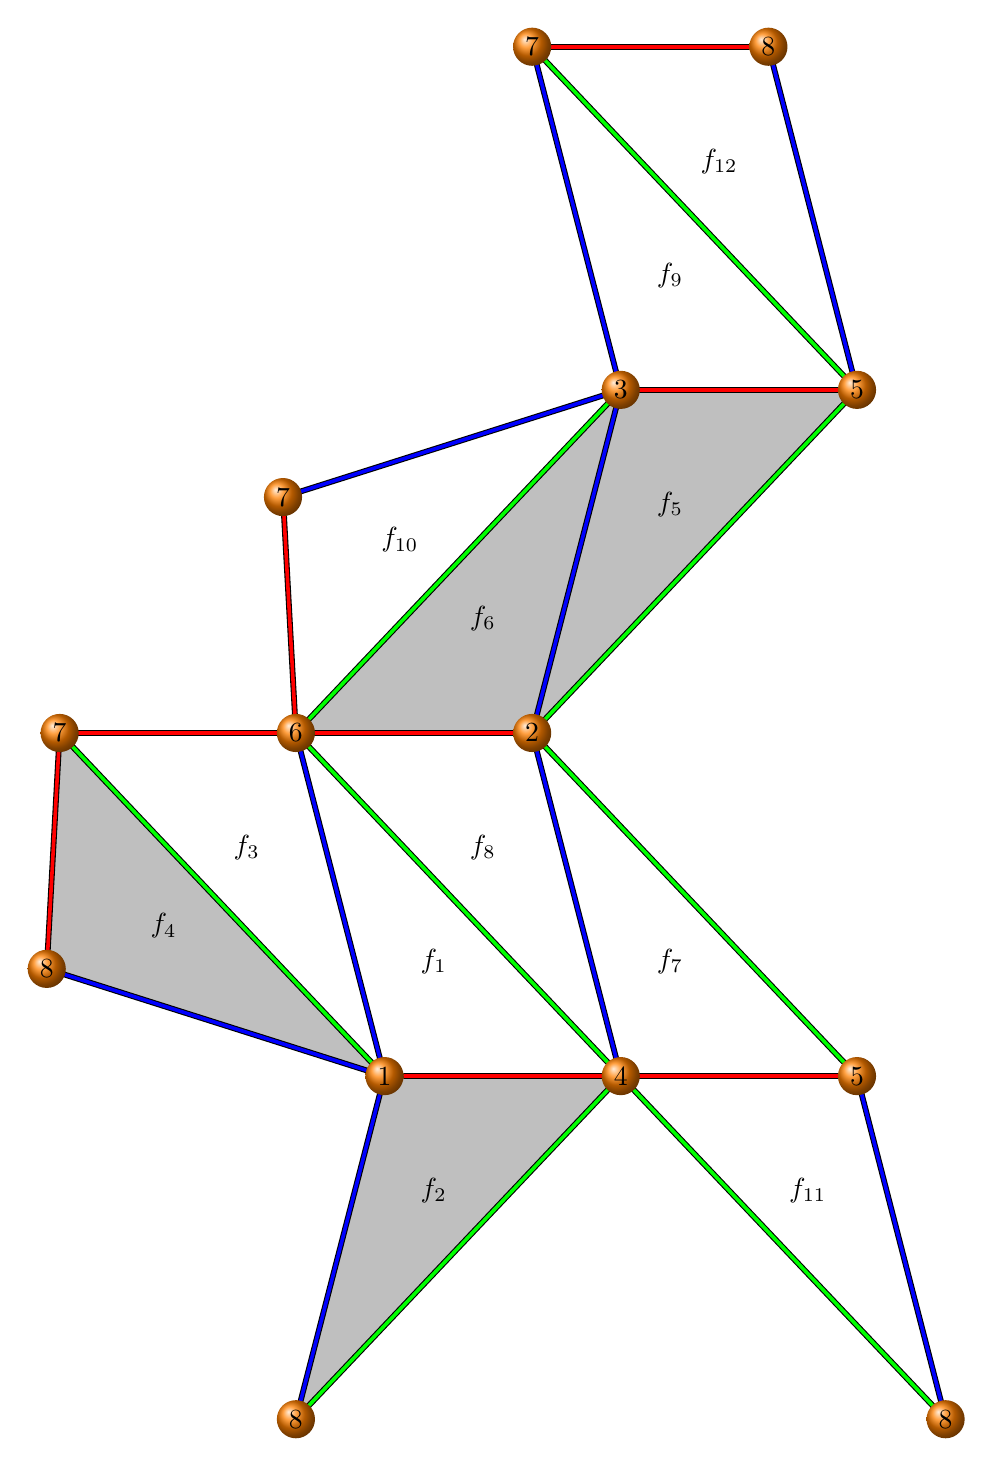
\begin{tikzpicture}[scale=3/2]
\coordinate (V1_1) at (0, 0);
\coordinate (V2_1) at (1.25, 2.904737509655563);
\coordinate (V3_1) at (2, 5.809475019311126);
\coordinate (V4_1) at (2, 0);
\coordinate (V5_1) at (4, 5.809475019311126);
\coordinate (V5_2) at (4, -4.440892098500626e-16);
\coordinate (V6_1) at (-0.75, 2.904737509655563);
\coordinate (V7_1) at (-0.859375, 4.901744547543762);
\coordinate (V7_2) at (-2.75, 2.904737509655563);
\coordinate (V7_3) at (1.25, 8.714212528966689);
\coordinate (V8_1) at (-0.75, -2.904737509655563);
\coordinate (V8_2) at (-2.859375, 0.9077304717673637);
\coordinate (V8_3) at (4.749999999999999, -2.904737509655563);
\coordinate (V8_4) at (3.25, 8.714212528966689);


\fill[white] (V1_1) -- (V4_1) -- (V6_1) -- cycle;
\node (F1) at (0.4166666666666666, 0.9682458365518543) {$f_{1}$};
\fill[lightgray] (V1_1) -- (V4_1) -- (V8_1) -- cycle;
\node (F2) at (0.4166666666666666, -0.9682458365518541) {$f_{2}$};
\fill[white] (V1_1) -- (V6_1) -- (V7_2) -- cycle;
\node (F3) at (-1.166666666666667, 1.936491673103709) {$f_{3}$};
\fill[lightgray] (V1_1) -- (V7_2) -- (V8_2) -- cycle;
\node (F4) at (-1.869791666666667, 1.270822660474309) {$f_{4}$};
\fill[lightgray] (V2_1) -- (V3_1) -- (V5_1) -- cycle;
\node (F5) at (2.416666666666667, 4.841229182759271) {$f_{5}$};
\fill[lightgray] (V2_1) -- (V3_1) -- (V6_1) -- cycle;
\node (F6) at (0.8333333333333333, 3.872983346207417) {$f_{6}$};
\fill[white] (V2_1) -- (V4_1) -- (V5_2) -- cycle;
\node (F7) at (2.416666666666667, 0.9682458365518541) {$f_{7}$};
\fill[white] (V2_1) -- (V4_1) -- (V6_1) -- cycle;
\node (F8) at (0.8333333333333333, 1.936491673103709) {$f_{8}$};
\fill[white] (V3_1) -- (V5_1) -- (V7_3) -- cycle;
\node (F9) at (2.416666666666667, 6.777720855862981) {$f_{9}$};
\fill[white] (V3_1) -- (V6_1) -- (V7_1) -- cycle;
\node (F10) at (0.1302083333333333, 4.538652358836817) {$f_{10}$};
\fill[white] (V4_1) -- (V5_2) -- (V8_3) -- cycle;
\node (F11) at (3.583333333333333, -0.9682458365518546) {$f_{11}$};
\fill[white] (V5_1) -- (V7_3) -- (V8_4) -- cycle;
\node (F12) at (2.833333333333333, 7.745966692414834) {$f_{12}$};


\tikzset{EdgeStyle/.style = {thin, double distance=1.3pt} }

\draw[ EdgeStyle, double=red] (V4_1) -- (V1_1);
\draw[ EdgeStyle, double=blue] (V1_1) -- (V6_1);
\draw[ EdgeStyle, double=green] (V1_1) -- (V7_2);
\draw[ EdgeStyle, double=blue] (V8_1) -- (V1_1);
\draw[ EdgeStyle, double=blue] (V1_1) -- (V8_2);
\draw[ EdgeStyle, double=blue] (V3_1) -- (V2_1);
\draw[ EdgeStyle, double=blue] (V2_1) -- (V4_1);
\draw[ EdgeStyle, double=green] (V5_1) -- (V2_1);
\draw[ EdgeStyle, double=green] (V2_1) -- (V5_2);
\draw[ EdgeStyle, double=red] (V6_1) -- (V2_1);
\draw[ EdgeStyle, double=red] (V3_1) -- (V5_1);
\draw[ EdgeStyle, double=green] (V6_1) -- (V3_1);
\draw[ EdgeStyle, double=blue] (V7_1) -- (V3_1);
\draw[ EdgeStyle, double=blue] (V3_1) -- (V7_3);
\draw[ EdgeStyle, double=red] (V5_2) -- (V4_1);
\draw[ EdgeStyle, double=green] (V6_1) -- (V4_1);
\draw[ EdgeStyle, double=green] (V4_1) -- (V8_1);
\draw[ EdgeStyle, double=green] (V8_3) -- (V4_1);
\draw[ EdgeStyle, double=green] (V7_3) -- (V5_1);
\draw[ EdgeStyle, double=blue] (V5_2) -- (V8_3);
\draw[ EdgeStyle, double=blue] (V8_4) -- (V5_1);
\draw[ EdgeStyle, double=red] (V6_1) -- (V7_1);
\draw[ EdgeStyle, double=red] (V7_2) -- (V6_1);
\draw[ EdgeStyle, double=red] (V8_2) -- (V7_2);
\draw[ EdgeStyle, double=red] (V7_3) -- (V8_4);



\tikzset{VertexStyle/.style = {
 shape = circle,
 ball color = orange,
 text = black,
 inner sep = 2pt,
 outer sep = 0pt,
 minimum size = 10pt} }

\node[VertexStyle] at (V1_1) {1};
\node[VertexStyle] at (V2_1) {2};
\node[VertexStyle] at (V3_1) {3};
\node[VertexStyle] at (V4_1) {4};
\node[VertexStyle] at (V5_1) {5};
\node[VertexStyle] at (V5_2) {5};
\node[VertexStyle] at (V6_1) {6};
\node[VertexStyle] at (V7_1) {7};
\node[VertexStyle] at (V7_2) {7};
\node[VertexStyle] at (V7_3) {7};
\node[VertexStyle] at (V8_1) {8};
\node[VertexStyle] at (V8_2) {8};
\node[VertexStyle] at (V8_3) {8};
\node[VertexStyle] at (V8_4) {8};

\end{tikzpicture}

\end{document} 
